\documentclass{IEEEtran}
\usepackage[utf8]{inputenc}
\usepackage{graphicx}
\usepackage{subcaption}
\usepackage{url}
\usepackage{amsmath}
\usepackage{wrapfig, framed, caption}
\usepackage{hyperref}
\hypersetup{
    colorlinks=true,
    linkcolor=blue,
    filecolor=blue,      
    urlcolor=blue,
    citecolor=blue,
    pdfpagemode=FullScreen,
    }
\usepackage{tabularx}
\usepackage{tabularray}
\usepackage[hmargin=1cm]{geometry}
\usepackage{multirow}

%Dissertation Checklist

%Finish Research Proposal (Few sections missing, sort out citations)
%Ethics Proposal (Done, need to sort out handbook citation)

%Questionnaire (Done)
%Data Analysis Method (Started)
%R-Code (Started)

%Quality Assurance Test Plan (Not Started)

%Presentation (Put hypothesis and more info on how the player model is created)

%Prototype (on defensive actions, check if nearby characters are attacking)

%Your document must not exceed six pages of text, excluding figures, tables, references and appendices.
%This is subject to the usual policy on word and page limits available on LearningSpace.


%Useful links
%G-Power downloads
    %https://www.psychologie.hhu.de/arbeitsgruppen/allgemeine-psychologie-und-arbeitspsychologie/gpower
    %https://learningspace.falmouth.ac.uk/mod/resource/view.php?id=245797

%\title{Evaluating the use of Adaptive AI to Build Player-Companion Collaboration} 
%Evaluating Collaboration With AI NPCs to Build Player-Companion Relationships
\title{Does the Use of Adaptive AI Help to Build Player-Companion Collaboration?}
\author{Andrew J. Scott}  
\date{September 2022}

\begin{document}
	\maketitle
	\pagenumbering{arabic}

\begin{abstract}
This proposal demonstrates the use of adaptive AI for companion characters that can work with players in an action game. The companion cannot be explicitly commanded, so the AI responds to player actions to collaborate with them better, which preserves independence. This adaption was tested to determine if the companion character gives the player a greater sense of teamwork.
\end{abstract}

 \begin{IEEEkeywords}
Artificial Intelligence, AI, Synergy, Collaboration, Cooperation, Companion, NPC, Adaptive, Game.
\end{IEEEkeywords}

\section{Introduction}
\label{Intro}

This research presents an AI companion that aids players in combat, similar to \textit{Atreus} in \textit{God of War} or \textit{Ellie} from \textit{The Last of Us}. The focus of this research is on using agent modelling, outlined in section \ref{Communication}, to make an adaptive AI that determines how the companion can best assist the player without requiring any explicit commands from them.

In the next section, this proposal summarizes the motivations for the project. In section \ref{RelatedWork}, this proposal analyses common design practices for AI. Sections \ref{Responsive Behaviour} \ref{Movement} \ref{ABC} focus on various methods for AI in industry, while section \ref{Communication} focuses on analysing methods in academic research that are used to create adaptive AI. Section \ref{ProposedResearch} details the design of the experiment used in this research. Section \ref{Artefact} demonstrates the AI technique used, the development of the artefact and quality assurance. Sections \ref{Results} \ref{Discussion} \ref{Further Work} \ref{Conclusions} analyse the results and evaluate the performance of the AI technique applied.

%Todo Mid: check sections

\section{Background}
\label{Background}

A key motivation for this work is a developer conference by Constantine et al. that focused on building the relationship between the players and their ally, Aurene, so that their death feels more meaningful \cite{EGXCharacterDeathGuildWars}. One of their points was that allowing players to explicitly command companions can ruin their agency.

When developing the AI for \textit{Atreus} in \textit{God of War}, there was a lot more of a focus on the sense of teamwork between Atreus and the player. This can be overshadowed as the player can explicitly command Atreus, which can ruin his agency \cite{EGXCharacterDeathGuildWars}. The intention for this research is to create an AI that can collaborate with the player like Atreus, but is independent like Aurene.

This research builds upon combat AI for companion characters by focusing on the sense of collaboration between them and the player while maintaining this independence. Collaboration in this research is defined as the sense of teamwork between the player and a companion NPC. This is built with synergistic behaviours where the AI makes it easier for the player to play the game in a noticeable way. To do this, this research presents an adaptive AI, which is where the companion will change their own behaviours in response to the player's actions. The intention is that responding to the player's actions will make them more collaborative.

The AI will have to balance multiple duties, such as helping the player stay safe, attacking other enemies so they do not get overwhelmed and maintaining their own safety \cite{CoupledEmpowermentMaximisation, tremblay2013adaptive}. To preserve player agency, the AI should not overshadow the player and will use mostly supportive behaviours to assist them \cite{DesignDocAIAllies}.

The combat actions for both the player and companion will be simple. This reduces scope and allows the AI to be incorporated in other action games easier. This is standard AI practice in industry \cite{GMTGoodAI, GDCLessIsMore, GDCSimplestAITrick}. While the player should be able to notice the AI, they should not need to rely on them for specific behaviours or completely change their play-style to get the AI to be helpful.

\section{Related Work}
\label{RelatedWork}

Research in 2010 highlights the lack of AI research in games \cite{RealTimeAICritique2010}. Since then, there has been a lot of improvements in AI research. Specifically looking at companion characters, there is a lot of research on implementing adaptive behaviour.

Friedman and Schrum analysed 2 companion bots in a first person shooter \cite{CompanionBotsFPS2019}. The ratings for the helpfulness of the companions was similar, which they said may have been due to vague terms. Adaptive agents that focus on being effective were rated as helpful due to the points they scored and their ability to survive better than non-adaptive AI. However, the non-adaptive agents that stayed near the player were also scored as helpful because they were seen in gameplay often. Players that rated the non-adaptive agents as more helpful justified this as they felt a stronger sense of teamwork and the game experience mattered more to them than points.

Geib et al. present a plan recognition approach that allows an agent to analyse the actions of another and use those actions to determine what plan is being attempted \cite{GeneratingCollabBehaviourPlanRecognition2016}. Unlike the agent by Friedman and Shrum \cite{CompanionBotsFPS2019}, this AI uses adaptive techniques to collaborate with another agent. This plan recognition agent adapts to the actions taken by another agent to determine their plan. Once a plan has been determined, the agent can work through the already completed steps to determine what still needs to be done and take actions towards these steps.

One of the more novel approaches, demonstrated by Tremblay and Verbugge, was to have a companion AI that can analyse the game intensity and change its behaviour as a way to dynamically adjust game difficulty \cite{tremblay2013adaptive}. Though this is not an example of AI adapting to another agent's actions, it still demonstrates the effect adaptability can have on the user experience.

In industry, games like \textit{God of War 2018}, \textit{The Last of Us} and \textit{Bioshock Infinite} are renowned for their AI companions \cite{PlayDontShow}. All three of the studios behind these games have developed AI techniques to fine-tune behaviour.

\subsection{Responsive Behaviour}
\label{Responsive Behaviour}

Atreus in \textit{God of War 2018} is a good example of synergistic AI, as he will help the player land slow attacks and will extend enemy vulnerability by shooting them with arrows \cite{GDCAtreus}. For example, when the player launches an enemy into the air, Atreus will shoot them and keep them there.

There is also a lot of emphasis on his character development over the course of the game, which is reflected in his behaviour. At the start of the game, he only takes actions when commanded, and learns to be more automated towards the middle of the game. Later, he becomes brash, so he starts to outright ignore the players’ commands, and performs actions that would otherwise only occur when commanded, like his special runic abilities.

These changes in his AI help to tie the narrative into game-play and make him seem like a real character, which helps to allow the player to bond with Atreus. These changes are also noticeable when the player is separated from Atreus, which helps the players realise how much they rely on him.

% TOTO - Include other sources that talk about responsive behaviours

\subsection{AI Movement}
\label{Movement}

%Image of pathfinding with caption
\begin{figure}
  \centering
  \includegraphics[width=\linewidth]{Images/IndustryResearch/TLOUPathfinding.png}
  
\caption{Pathfinding diagram in \textit{The Last of Us}}
\label{fig:TLOUPathfinding}
\end{figure}

Pathfinding is an important aspect of AI companions. The AI needs to be close to the player so that it is not forgotten \cite{GAIP2EllieAI}, but also not too close that it gets in their way and obstructs them \cite{CoupledEmpowermentMaximisation}. An example of poor AI pathfinding is in \textit{Skyrim} \cite{tremblay2013adaptive}, where the AI will move in front of the player when they are aiming and generally get in their way when moving. Naughty Dog addressed issues like this in \textit{The Last of Us} with pathfinding tools, shown in figure \ref{fig:TLOUPathfinding}, that keeps companions close to the player, but not in the way \cite{GAIP2EllieAI}. Ellie will also move out of the way if the player moves into her personal space. Vocal barks are used in such moments to add character, and it is a good practice to use voice acting to help make the player aware of the agent’s actions, and make them feel more real \cite{GMTGoodAI}. However, they may not be suitable for games with lower budgets.

%Images of fight circles with captions
\begin{figure}
  \centering
  
  \begin{subfigure}[a]{\linewidth}
  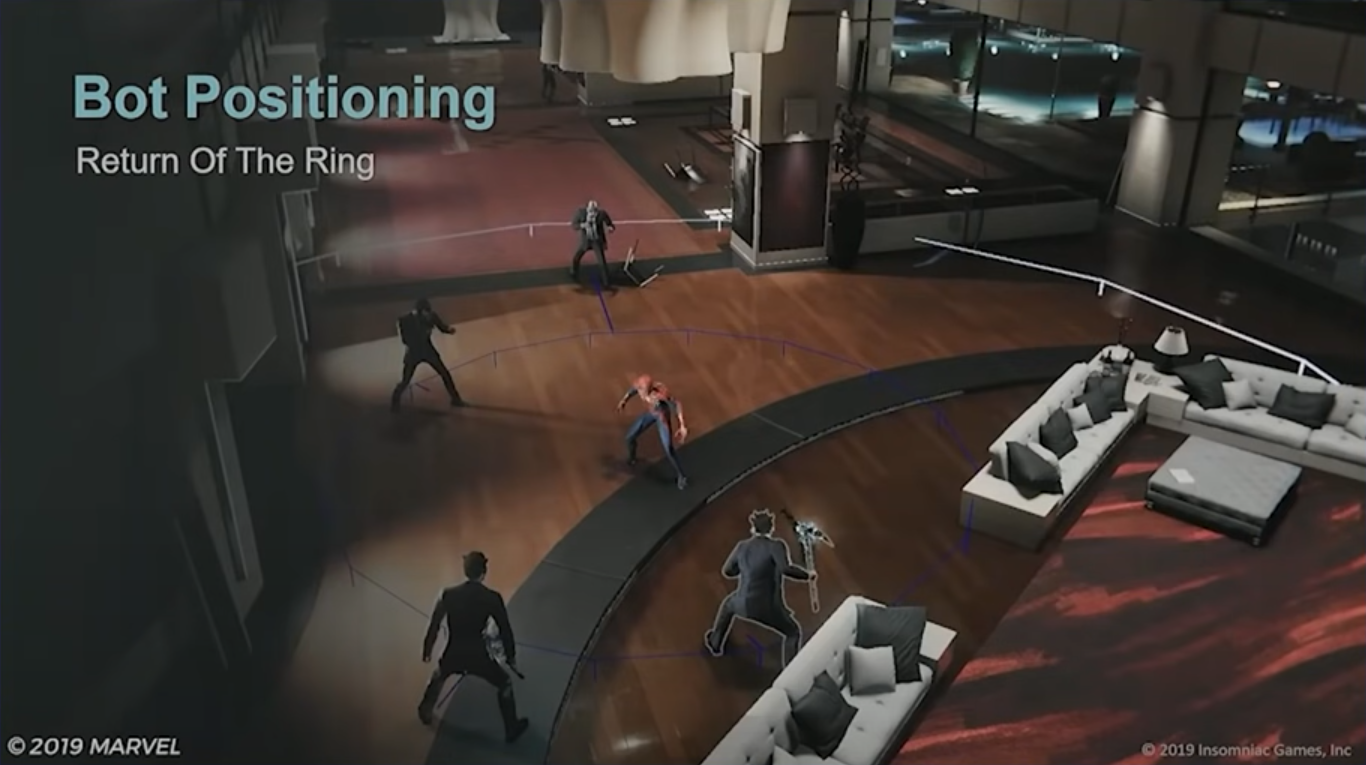
\includegraphics[width=\linewidth]{Images/IndustryResearch/SpidermanKungFuCircle.png}
  \end{subfigure}
  
  \begin{subfigure}[b]{\linewidth}
  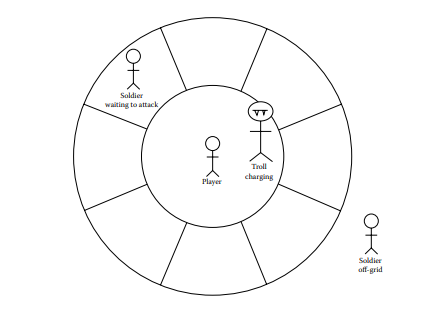
\includegraphics[width=\linewidth]{Images/IndustryResearch/KOARKungFuCircle.png}
  \end{subfigure}
  
  \caption{Demonstration of Kung-Fu Circles in (a) \textit{Marvel's Spiderman} and (b) \textit{Kingdoms of Amalur: Reckoning}}
  \label{fig:KungFuCircle}
\end{figure}

Many action games, such as \textit{Marvel's Spiderman} and \textit{Kingdoms of Amalur: Reckoning}, use a technique known as the Kung-Fu Circle to manage the positioning of multiple agents \cite{GAIPKungFuCircle, GDCSpiderman}, shown in figure \ref{fig:KungFuCircle}. An AI manager handles the positioning of enemies in this circle and manages when they can attack. While this technique is intended to manage multiple enemies in action games, it can be used to determine where the AI companion could be placed.

\subsection{Animations, Bespoke Behaviours and Call-outs}
\label{ABC}

A lot of industry practice with developing AI for companion characters is to use bespoke behaviour, detailed animations and vocal call-outs to give personality and character \cite{GAIP2EllieAI, GMTGoodAI, GAIPOReactions}. In particular, Irrational Games created a smart terrain system for \textit{Bioshock: Infinite} that allows \textit{Elizabeth} to interact with the environment \cite{GDCElizabeth, AIGamesBioshockAI}, shown in figure \ref{fig:BioshockSmartTerrain}. A lot of these finishing touches are a key part of making the companion feel more believable, allowing the player to empathise and engage with them more. It also helps to communicate NPC actions, so the player understands that they are actually making choices, otherwise they can miss the intelligence of the AI \cite{GMTGoodAI}.

Instead of focusing on animation and voice lines, the agent will use adaptive AI to improve the sense of collaboration between them and the player. The intent of this would be to improve player-companion relationships in games with lower budgets and to maximise them in games that can have animations and voice acting. To do this, it will feature AI techniques that allow a companion NPC to adapt to player actions to collaborate with them better.

\begin{figure}
  \centering
  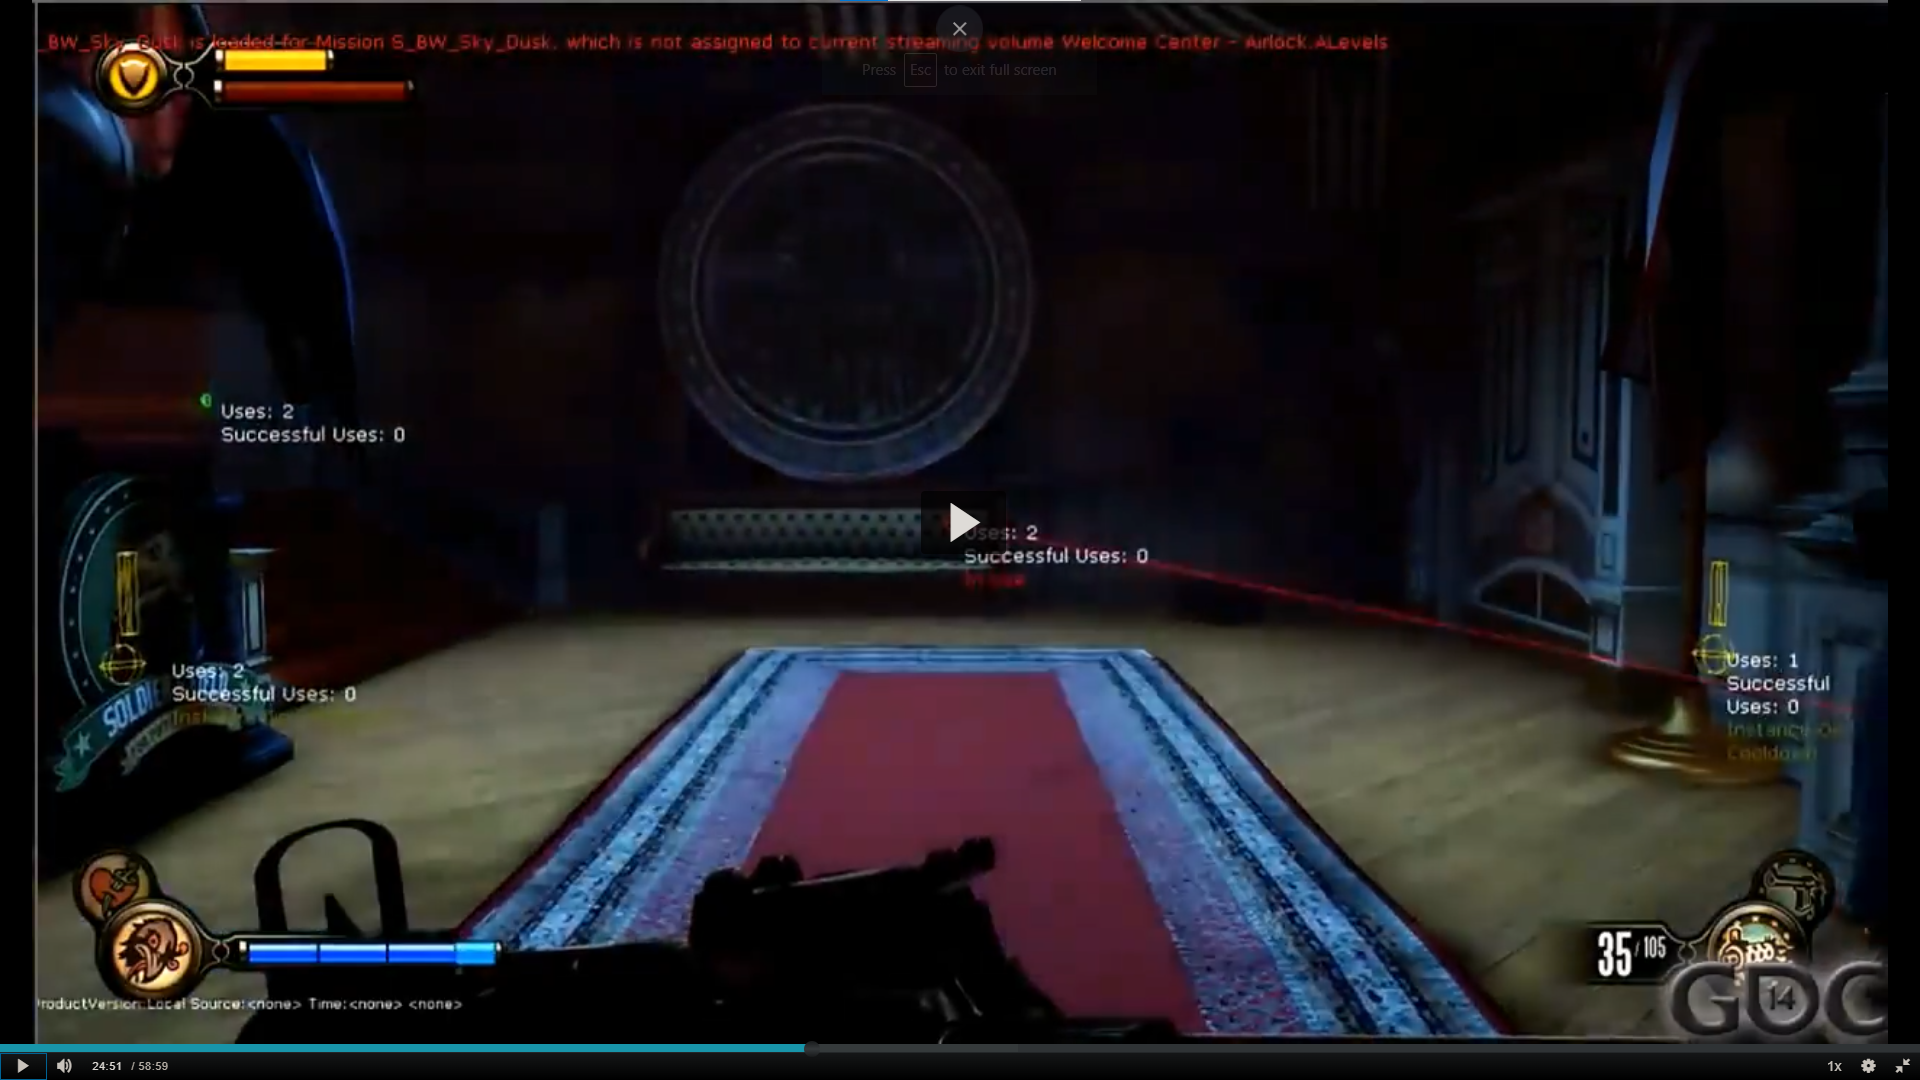
\includegraphics[width=\linewidth]{Images/IndustryResearch/BioshockSmartTerrain.png}
  
\caption{Smart Terrain showcase in \textit{Bioshock: Infinite}}
\label{fig:BioshockSmartTerrain}
\end{figure}

\subsection{Collaboration Without Communication}
\label{Communication}

The core design, detailed in Section \ref{Background}, is that the player cannot explicitly command the companion. As a result, the AI needs to determine how to collaborate with the player without communication. The following methods are some ways in which an AI can collaborate with other agents without communication.

Board games like \textit{Hanabi} and \textit{Pandemic} are often used in academic research for collaborative AI as they involve teamwork between multiple players that cannot communicate with each-other. Eger and Grus demonstrate a technique for \textit{Hanabi} that uses timing to communicate between agents \cite{WaitASecond2019}. While this is effective for collaboration between AI agents, this method is not reliable for player-AI collaboration as a human player isn't going to perform actions at specific timings to communicate with an AI agent.

Walton-Rivers et al. present a an AI for \textit{Hanabi} that uses agent modelling to collaborate with other AI players \cite{EvaluatingHanabiAgents}. Agent modelling techniques involve observing actions taken by a player or another agent and using these actions to construct a model of them. This model describes how the observed entity acts and can be used by the AI determine its actions. Yannakakis et al. demonstrate the use of machine learning to determine how an agent can use a player model \cite{yannakakis2013playermodelling}.

Agent modelling can also be used in Real-Time Strategy (RTS) games. Schadd et al. demonstrate the use of agent modelling for \textit{Spring} \cite{OpponentModellingRTS2007}. Bakkes et al. then build upon this research to use it in Case-based game AI \cite{bakkes2009opponentmodelling}.

%\cite{van2005opponent} - This tends to not be used for commercial games however (though this source is from 2005 so it may be out of date)

Plan recognition is another common technique that is used in board games. This is another technique for agents that need to collaborate with other agents, including players, without requiring explicit commands or communication. Agents that use plan recognition observe the actions, similar to agent modelling. However, instead of constructing a model of the player, it uses these actions to their goals by comparing the steps required to achieve that goal to the steps that have been taken \cite{GeneratingCollabBehaviourPlanRecognition2016}. Once an entity’s goal has been identified, the plan recognition agent will devise actions that can aid them in achieving their goals. The unfinished steps in the plan can be used as potential behaviours.

Sauma-Chacón and Eger evaluate the use of plan recognition agents in \textit{Pandemic} that can play with a human player \cite{PandemicPlanRecognition2021}. This AI was able to play at a level similar to that seen in full teams of AI and was perceived as more helpful. In addition, they detected a correlation between perceived helpfulness and skill.

Like agent modelling, this technique can also be used in RTS games as agents use observed behaviour to determine their allies' or opponents' plans. Jansen demonstrates the use of plan recognition as an ally in RTS games, instead of using it as an opponent \cite{PlayerAdaptiveRTSAI2007}. This agent can look at the player's actions and build units to support their plans.

\section{Proposed Research}
\label{ProposedResearch}

\subsection{Research Question \& Hypotheses}
\label{Hypotheses}

The use of adaptive AI companions can have an effect on various aspects of the game-play. The main aspect this research tests for is creating a sense of collaboration between the player and companion agent during combat and the question this research attempts to answer is \textit{Does the use of adaptive AI help to build player-companion collaboration?}

This question is the focus of the first hypothesis; the adaptive AI will be perceived as more collaborative than the non-adaptive AI. This will be tested in the experiment detailed in section \ref{ExperimentalDesign}. Comparing the rankings for the collaboration of both agent types using a T-test will determine if the behaviours result in a greater sense of collaboration.

The null hypothesis here is that adaptability has no discernible effect on the player's perception of collaboration or that it is rated as less collaborative. This will be determined if there is no significant correlation, or a negative correlation, between the agent type and the rankings for collaboration.

The second hypothesis is that there will be a correlation between the rankings for the participants’ sense of collaboration and user experience. In an experiment by Friedman and Schrum, more detail in section \ref{RelatedWork}, some players rated the non-adaptive AI as more helpful was that it was seen more in game-play, even if it scored lower in game \cite{CompanionBotsFPS2019}. Players justified this as it gave them a better player experience and sense of teamwork. A correlation test between the user experience and collaboration ratings is used to test this.

\begin{tabular}{ |p{0.3cm}|p{2.5cm}|p{2.5cm}|p{1.8cm}|  }
 \hline
 \multicolumn{4}{|c|}{Hypothesis Table} \\
 \hline
 No. & Hypothesis & Null Hypothesis & Test\\
 \hline
    1 & Adaptive companion will be seen as more collaborative compared to the non-adaptive companion & 
    The adaptive agent is not rated as more collaborative than the non-adaptive agent &
    T-Test between the collaboration ratings of both agent types \\
 \hline
    2 & Players' user experience will be improved if they felt a greater sense of collaboration & 
    There is a negative or no correlation between user experience and their sense of collaboration &
    Correlation test between the user experience and collaboration ratings\\
 \hline
\end{tabular}

\section{Artefact}
\label{Artefact}

\subsection{Artefact Details}
\label{ArtefactDetails}

This research presents an adaptive AI for an action game responds the the player actions to collaborate with them. The intention is that this collaboration will improve the player experience, and this is one of the factors that is tested, see section \ref{Hypotheses} for details on the hypotheses.

The agent has general path-finding behaviours that keep it close to the player or enemy targets and it will try to stay within their vision so the player notices it. The AI features a behaviour tree to determine its tasks. the tasks mostly involve staying near the player and attacking nearby enemies.

This agent features agent modelling, detailed in \ref{Communication}. When the player performs a combat action, the adaptive AI will be given information about what kind of action the player took and whether they were successful. It uses this information to construct a model that describes how the player acts. This model is made up of key descriptors that describe the player's actions.

Every time the player takes an aggressive action, such as attacking, the AI will add to aggressive descriptor. However, if they miss, the AI will add to a panic descriptor. Each action will add to a specific descriptor and the amount they add will be tweaked in play-testing, see appendix \ref{AppendixQAPlan}. It will then use this player model in behaviour tree when deciding what it will do.

For example, if the player is aggressive, but are getting hit a lot, the companion AI may use flanking behaviours to attempt to draw enemies away from the player so they can focus on fewer targets. However, if the player is very defensive, and tends to attack only after an enemy attacks, the adaptive AI may focus on the player's current target and create an opening for them to attack. If the player is getting overwhelmed by enemies, the agent may try to draw enemies away from the player to give them some space to relax or it will intercept themselves between the player and their enemies.

A plan recognition approach would have required the player to think about their strategy more, which would suit a slower or more strategic game. An action game is faster paced, and because the player does not have as much time to think, they won't be able to come up with plans. As a result, this project will feature a player modelling approach because it can work better with a simpler combat system, but still enables adaptive behaviour.

\subsection{System Development Life-cycle}
\label{DevLifecycle}

The project uses version control to track changes. In addition, a task board has been made, and will be used to track the progress of the development.

The initial prototype (commit: \url{https://github.falmouth.ac.uk/Games-Academy-Student-Work-22-23/Buddy-NPC-Dissertation/commit/493e0063025132e950696b4d174af48a5b190060}) features a basic combat system. The player can move, attack, parry and dodge and these basic mechanics were not changed much in later commits. The AI agents in this commit use the update loop instead of a behaviour tree, and chase their closest enemy and attack when they are in range.

The agent modelling is in a prototype state in this commit, and does not affect the agents' actions. The agent modelling script can observe actions performed by a specified character assign a basic descriptor that defines their dominant play-style.

The prototyped was refactored (commits: \url{https://github.falmouth.ac.uk/Games-Academy-Student-Work-22-23/Buddy-NPC-Dissertation/commit/ff3c28e4a07d2bb3549c6dbc93962801a3e29a72} and onward). Subsequent commits implemented a behaviour tree, which allows for easier modification and extension to the AI. The AI agents were also being designed. Commits after this point are labeled “feat: Basic AI”, “feat: Adaptive AI”, “feat: Interval AI” or “feat: General AI” to show which agent was being developed.

Some of the key mechanics and changes that emerged from the development included flanking and intercepting behaviour. The original plan was to have the adaptive agent flank when the player is performing counter attacks against the AI. However, this did not produce much of a difference compared to normal movement, since it would usually move behind the enemy anyway.

However, it did produce behaviour that resulted in it drawing enemies away from the player, which was more suited to if the player was struggling so this behaviour was moved to the panicking model instead of the counter model. Now, when the player is dodging a lot, the AI will rush to the player and attempt to draw enemies away from them so they can focus on parrying attacks or countering.

%TODO Mid: change comments in project to reflect dodge behaviour better

When designing unit tests for the \textbf{GetFlankPosition} function, it was discovered that passing in a negative value for the distance would return a position between the targets. From this, a new behaviour emerged for the AI. With some small tweaks to the flanking behaviour, a new behaviour was made where the agent will position itself between the player and their enemies, which is used to protect them. this is used when the player is panicking.

\subsection{Validation and Verification}
\label{Validation}

The original QA plan can be found in appendix \ref{AppendixQAPlan}. The main changes from this plan were the order in which tests were conducted and some tests were removed because they were unnecessary.

\subsubsection{Unit Testing}

Unit tests were derived for certain calculations to ensure that they were correct. Most commits tagged “chore: Maintainability” implement unit tests.

The first set of unit tests are edit mode tests that asserts the flank position helper function (commit: \url{https://github.falmouth.ac.uk/Games-Academy-Student-Work-22-23/Buddy-NPC-Dissertation/commit/489e9531dc36e221bb54ee781e269374bceb39fb}). It passes a series of vectors through the function and confirms that they are almost equal (threshold = 0.1) to the expected value. Doing these tests also presented the idea of implement an intercept behaviour, where the agent will position itself between the player and their enemies to help protect them.

Most of the unit tests were for play mode. The first set of play mode unit tests were designed to test the model generator script (commit: \url{https://github.falmouth.ac.uk/Games-Academy-Student-Work-22-23/Buddy-NPC-Dissertation/commit/79fbfa4363a7fd344704371576a393296f90e5fa}). These tests assert that taking actions will generate the correct player model and it does so independently of the combat scripts, so it only checks the model script.

Expanding on this, unit tests for the combat script were developed (commit: \url{https://github.falmouth.ac.uk/Games-Academy-Student-Work-22-23/Buddy-NPC-Dissertation/commit/1025827dfae1c7f332cd65cad784253b0f5a128d}). These tests extend these checks by determining that the model is generated correctly from actions within the combat script. These tests found an issue with the attack, dodge and parry actions, which would cause the model to think the player is panicking. These occurred from a function within these actions where they would end the current attack, which causes the model to think that the character made an attack. This issue was then fixed (commit: \url{https://github.falmouth.ac.uk/Games-Academy-Student-Work-22-23/Buddy-NPC-Dissertation/commit/4b13e199a2f760e0d2574d523f242cbd5197f62f}).

The final unit tests focus on the health scripts (commits: \url{https://github.falmouth.ac.uk/Games-Academy-Student-Work-22-23/Buddy-NPC-Dissertation/commit/e6c5556d8516e4dbd2ed21b37efe5b969676a921} and \url{https://github.falmouth.ac.uk/Games-Academy-Student-Work-22-23/Buddy-NPC-Dissertation/commit/d54f7006788c28840f9907d52d115ef12389be85}). These commits assert that the health is correctly calculated from damage taken and healing received. It also checks that the player should be killed if they receive damage that brings their health below 0. Additionally, the second commit contains a change that prevents healing above max health by clamping the health value.

\subsubsection{Integration Testing}

During the development of the artefact, incremental integration testing was used to ensure individual elements were implemented properly.

The initial prototype (commits: \url{https://github.falmouth.ac.uk/Games-Academy-Student-Work-22-23/Buddy-NPC-Dissertation/commit/493e0063025132e950696b4d174af48a5b190060} and earlier) focus on the player mechanics and the character animations. The AI implemented in this prototype had some of the basic behaviour needed to test the combat mechanics. The AI for both the companion and enemies did not use a behaviour tree in this prototype, instead using the update function to determine actions.

The player model in the initial prototypes also had no influence on the companion's behaviour in this initial prototype, but it was implemented and the player state was displayed on the UI to test how player actions influenced it.

There are also various scenes within the project that are used to test specific mechanics. For example, scenes where the health is set extremely high for all characters to focus on testing AI changes in combat, and a scene with just the player and an enemy is used to refine combat mechanics. Commits \url{https://github.falmouth.ac.uk/Games-Academy-Student-Work-22-23/Buddy-NPC-Dissertation/commit/ff11d5391f1061188ef66f10168e92f57260a6f6} and \url{https://github.falmouth.ac.uk/Games-Academy-Student-Work-22-23/Buddy-NPC-Dissertation/commit/cbe07de2fea626ece57619bfa3662d25ab53ce1d} show some changes based on this testing.

\subsubsection{System Testing}

These behaviours were tested with pilot play-testing with verbal feedback to ensure that the player model is constructed properly and that appropriate actions are taken based on the current player state. From this initial play-testing, players were struggling with the high difficulty as enemies would swarm the player and constantly attack them. This high difficulty was intended to force the player to rely on cooperating with their ally, but players found it too stressful to notice the AI.

The combat difficulty was reduced by making changes to the enemy AI to reduce swarming behaviours (commit: \url{https://github.falmouth.ac.uk/Games-Academy-Student-Work-22-23/Buddy-NPC-Dissertation/commit/8b6b4494752d3c8ff0bd402af97b4a65a13a5d77}). This commit added a cooldown between attacks and adjustments to the enemy AI to move enemies away in a small circle if they cannot attack, similar to the Kung-Fu circle method used in \textit{Kingdoms of Amalur: Reckoning} \cite{GAIPKungFuCircle}. This reduced frustration and stress while allowing the player to notice their companion more.

In addition, various quality of life changes were made to the camera, UI, inputs and attack animations to make the game more intuitive and accessible.

\section{Research Method}
\label{ResearchMethod}

\subsection{Philosophical Position}
\label{PhilosophicalPosition}

%What is this thing called Science? https://falmouth.primo.exlibrisgroup.com/discovery/fulldisplay?context=L&vid=44FAL_INST:44FAL_VU1&search_scope=MyInst_and_CI&tab=Everything&docid=alma9911072374905136
%Scientific Method https://plato.stanford.edu/entries/scientific-method/
%Philosophy of Science https://undsci.berkeley.edu/the-philosophy-of-science/
%Philosophy and Paradigm of Scientific Research https://www.intechopen.com/chapters/58890 

%TODO Low - research empirical philosophy to see if it fits better
% TODO Low Justify philosophies

The research was carried out using positivist philosophies \cite{Zukauskas18}. A survey was used to collect quantitative data that analyses the effect of AI adaptability on the player's collaboration the AI agent, and how that affects their opinions on the AI. There were some questions with qualitative answers, but these were used to assure that there are no issues with the study.

\subsection{Experimental Design}
\label{ExperimentalDesign}

%Might be best to have each participant play both as they could be skewed by personal biases so the baseline needs to be established randomise the order

%G-Power video explanation: https://web.microsoftstream.com/video/d1ec1c56-bb97-4592-ae4e-1c973e3fee20?referrer=https:%2F%2Flearningspace.falmouth.ac.uk%2F

The experiment took place on campus at the Games Academy Warehouse.

Two companion agents were set up in an action game. The Agent Modelling (AM) companion uses player actions to calculate which state the player is in, and uses a behaviour tree to determine which actions to take based on this state. AM will determine targets based on the player actions and choose behaviours that support their intentions better.

The original plan was to test the AM agent against the simple AI already implemented in the initial prototype, see section \ref{DevLifecycle} for more details. However, during development it was decided that this would not be a fair experiment as the simple AI does not have access to the same behaviours. As such, the Interval Timing (IT) agent was developed to properly test the AM agent. The IT agent has access to the same behaviours, but instead of using the player state through the player actions, it randomly changes between states every 3-8 seconds.

Participants played through a demo that features a tutorial and two combat encounters. In one encounter, the participant will be assisted by the IT agent, while the other encounter will have them assisted by the AM agent. To avoid observer bias, the order the agents feature will be randomly selected \cite{hrobjartsson2013observer}. Once they have played through the demo, the participants were given a questionnaire form to fill out.

There is a link to the questionnaire in appendix \ref{AppendixLinks}.

\subsection{Data Management Plan}
\label{DataManagement}

%Data management and questionaire

Most of the questions use a Likert scale to distil responses into quantitative data and will include questions on how likeable, intelligent, collaborative, etc. the player thought they were, using a similar approach used by Z. Ashktorab et al. \cite{SocialPerceptions2020}. There will be some qualitative questions that allow participants to put sentence answers so they can give more specific thoughts. This will also help to determine if there are any bugs that caused one AI to not work as intended.

% TODO Low: Cite likert scale central tendency

The questions will use a 7-point Likert scale. Using a 7-point scale gives more accuracy as it reduces a central tendency bias. This is caused when participants avoid choosing extreme responses to avoid seeming like they have extremist values.

The questionnaire is linked in appendix \ref{AppendixLinks}. The responses to this were converted to a csv file, and stored on an online network drive. This data was analysed using R Studio, outputing various graphs that visualised the data for readers and statistical tests were conducted to assert the hypotheses, detailed in section \ref{Hypotheses}. The R-Code is in appendix \ref{AppendixRCode}.

Using G-Power, a sample size of 59 is required for T-Tests with an effect size of 0.4. This effect size was chosen because it is a medium-large effect size, as defined by Cohen \cite{cohen1988statistical}. A small or medium effect size may not be noticed by most players, especially in a fast-paced action game, as they may be more focused on their own behaviours.

%G-Power downloads
    %https://www.psychologie.hhu.de/arbeitsgruppen/allgemeine-psychologie-und-arbeitspsychologie/gpower
    %https://learningspace.falmouth.ac.uk/mod/resource/view.php?id=245797

\subsection{Ethical Considerations}
\label{EthicalConsiderations}

The data collection involved an experiment that focuses on various AI behaviours, and how different behaviours can build a stronger emotional connection between players and AI companion NPCs. As such, participants were involved. Participants tested the AI and filled out survey forms to give their opinions on the various AI mechanics. Under these criteria, there are no high risk categories, but since participants are involved, it counted as a medium risk experiment. The Nuremberg Code, the Falmouth University guidelines and the BCS Code of Conduct have been followed to protect the rights of the participants \cite{germany1949trials, BCSConductCode}.

The participants were given information forms that detail the experiment and their participation in it. There are no aspects of the experiment that are hidden from the participants, and the form has clear information on what the experiment will entail. The form has information on the purpose of the research, expected duration, procedures, what the participants are being asked to do, their right to decline and withdraw, confidentiality and contact info for the researcher.

In order to participate within the experiment, the participant were asked to sign that they understand and agree with the form, no signature will be required as it is an online form. Participants will also be required to state that they are at least 18 years of age to participate with the experiment. However they will not need to state their age, only that they are above 18 years old. There will also be no transactions or other coercion to participate with the experiment.

All participants will be given a right to withdraw at any time and this will also be made clear in the information and consent forms. The forms will have contact information for them and a reference number so that their responses can be removed without requiring them to give any personal information. They will also be able to use this number to check their responses, though they will not be able to change their responses once submitted to preserve pure data, they can only be removed.

The questions on the survey forms do not have any questions that require the user to input personal information. The questions are focused on their opinions of the AI.

Most of the questions use a Likert scale, and there are a few qualitative questions that allow them to express more opinions. None of the questions require the participants to divulge any personal information. Once the data has been analysed, it will be archived until the study is complete, after which all responses will be deleted.

\section{Results}
\label{Results}

59 people participated in the playtesting sessions. Of those 59 participants, 4 of their survey responses had to be removed because their forms were filled out incorrectly. This left 55 valid responses, each of which had 2 data points. In addition to the 2 hypotheses detailled earlier, additional tests were carried out to test 2 posthoc hypotheses.

%TODO Mid: more detail on invalid surveys

\begin{tabular}{ |p{0.3cm}|p{2.5cm}|p{2.5cm}|p{1.8cm}|  }
 \hline
 \multicolumn{4}{|c|}{Hypothesis Table} \\
 \hline
 No. & Hypothesis & Null Hypothesis & Test\\
 \hline
    1 & Adaptive companion will be seen as more collaborative compared to the non-adaptive companion & 
    The adaptive agent is not rated as more collaborative than the non-adaptive agent &
    T-Test between the collaboration ratings of both agent types \\
 \hline
    2 & Players' user experience will be improved if they felt a greater sense of collaboration & 
    There is a negative or no correlation between user experience and their sense of collaboration &
    Correlation test between the user experience and collaboration ratings\\
 \hline
    P1 & Players' user experience will be improved if they felt a greater sense of collaboration & 
    There is a negative or no correlation between user experience and their sense of collaboration &
    Correlation test between the user experience and collaboration ratings\\
 \hline
    P2 & Players' user experience will be improved if they felt a greater sense of collaboration & 
    There is a negative or no correlation between user experience and their sense of collaboration &
    Correlation test between the user experience and collaboration ratings\\
 \hline
\end{tabular}

\subsection{Hypothesis 1 - The adaptive companion will be perceived as more collaborative than the non-adaptive companion}

This hypothesis evaluates the players’ perception of collaboration between both agent types. A t-test between the collaboration ratings of both agent types returns a p-value of 0.2889. This high value means that it is possible that the null hypothesis is true.

\begin{figure}
  \centering
  \includegraphics[width=\linewidth]{Images/Graphs/H1CollabBox.pdf}
  
\caption{Box chart displaying each agents' user ratings for the collaboration}
\label{fig:H1CollabBox}
\end{figure}

\begin{figure}
  \centering
  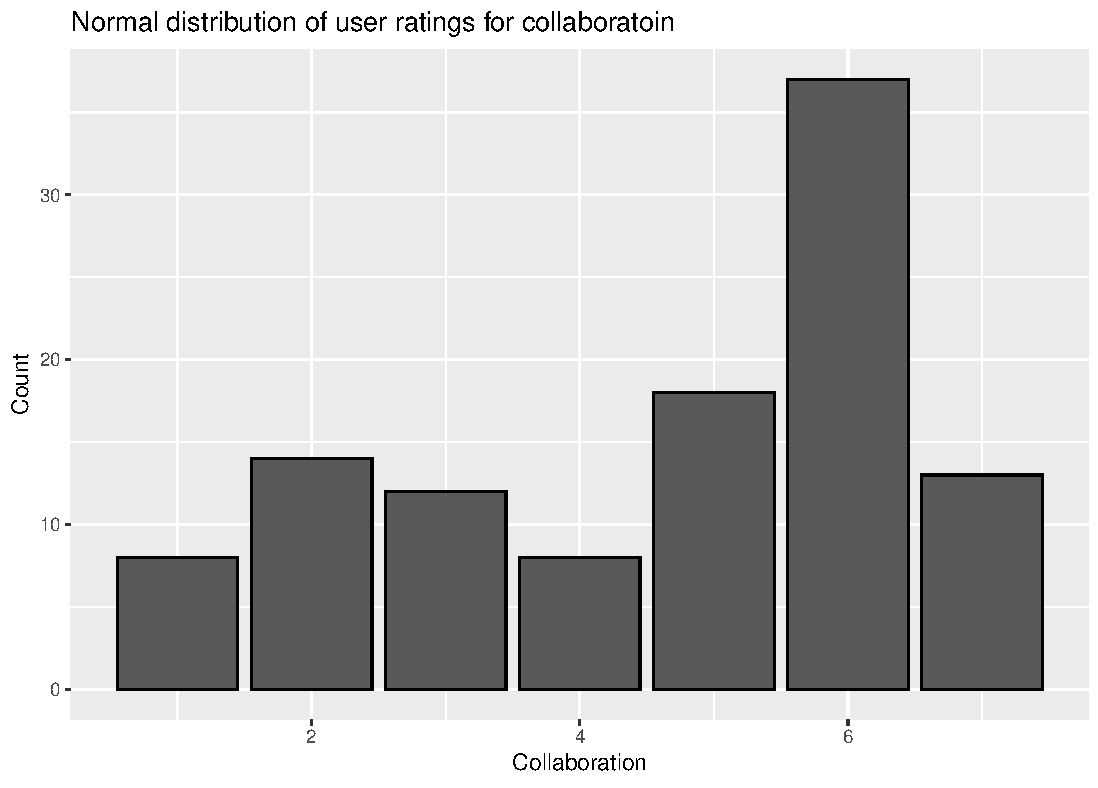
\includegraphics[width=\linewidth]{Images/Graphs/H1CollabBar.pdf}
  
\caption{Bar chart displaying the distribution of collaboration ratings across both companions}
\label{fig:H1CollabBar}
\end{figure}

\begin{figure}
  \centering
  \includegraphics[width=\linewidth]{Images/Graphs/H1CollabPairBar.pdf}
  
\caption{Pairwise comparison bar chart displaying the difference in user ratings for collaboration}
\label{fig:H1CollabPairBar}
\end{figure}

As shown in figures \ref{fig:H1CollabBox} and \ref{fig:H1CollabBar}, there is very little difference in the collaboration ratings for each agent type. Additionally, a pairwise comparison shows that most players did not perceive a difference between agent types, as shown in figure \ref{fig:H1CollabPairBar}. In this graph, the ratings for each player were subtracted to show the differences between their ratings for each companion. Most of the players rated each companion equally, resulting in a difference of 0.

\subsection{Hypothesis 2 - Players' user experience will be improved if they felt a greater sense of collaboration}

This hypothesis evaluates the correlation between the collaboration ratings and how much players enjoyed playing with that agent. A correlation test between these ratings returns a p-value less than 0.05 and a correlation of 0.4790956. This low p-value indicates that the null hypothesis may be false, however there is only a modest correlation between sense of collaboration and user experience.

Figure \ref{fig:H2CollabUXScatter} shows a scatter plot that demonstrates the user ratings, and a colour scale has been added to show how many participants rated each combination. This shows a weak correlation between the ratings, but as their sense of collaboration increases, so does their rating for how much they enjoyed playing.

\begin{figure}
  \centering
  \includegraphics[width=\linewidth]{Images/Graphs/H2CollabUXScatter.pdf}
  
\caption{Scatter plot displaying the correlation between collaboration and how much they enjoyed playing}
\label{fig:H2CollabUXScatter}
\end{figure}

\subsection{Post-hoc Test 1 - Players will rate their agent as more collaborative if they thought they were more adaptive}

This test was used to evaluate how effective the use of adaptive behaviour is at fostering a sense of collaboration.

A correlation test between these ratings returns a p-value les than 0.05 and a correlation of 0.516152. There is a modest correlation between the ratings for adaptivity and collaboration, which could indicate that if the player perceived the agents as adapting to their behaviour, then they also collaborate with the player better as well.

Figure \ref{fig:PH1AdapCollabScatter} shows a scatter plot that demonstrates the user ratings for adaptivity and collaboration. This shows a modest correlation between the ratings between adaptivity and collaboration.

\begin{figure}
  \centering
  \includegraphics[width=\linewidth]{Images/Graphs/PH1AdapCollabScatter.pdf}
  
\caption{Scatter plot displaying the correlation between adaptivity and collaboration}
\label{fig:PH1AdapCollabScatter}
\end{figure}

\subsection{Post-hoc Test 2 - Players will rate their agent as more believable if they thought they were more intelligent}

This test was used to evaluate the effect perceived intelligence has on how believable the agents were. A correlation test between these ratings returns a p-value less than 0.05 and a correlation of 0.6011652. There is a modest correlation between the ratings for intelligence and believability, which could indicate that increased intelligence ratings lead to the agents being perceived as more believable. A scatter plot for intelligence and believability ratings does not show a strong correlation between intelligence and believability, as shown in figure \ref{fig:PH2IntelBelieveScatter}.

\begin{figure}
  \centering
  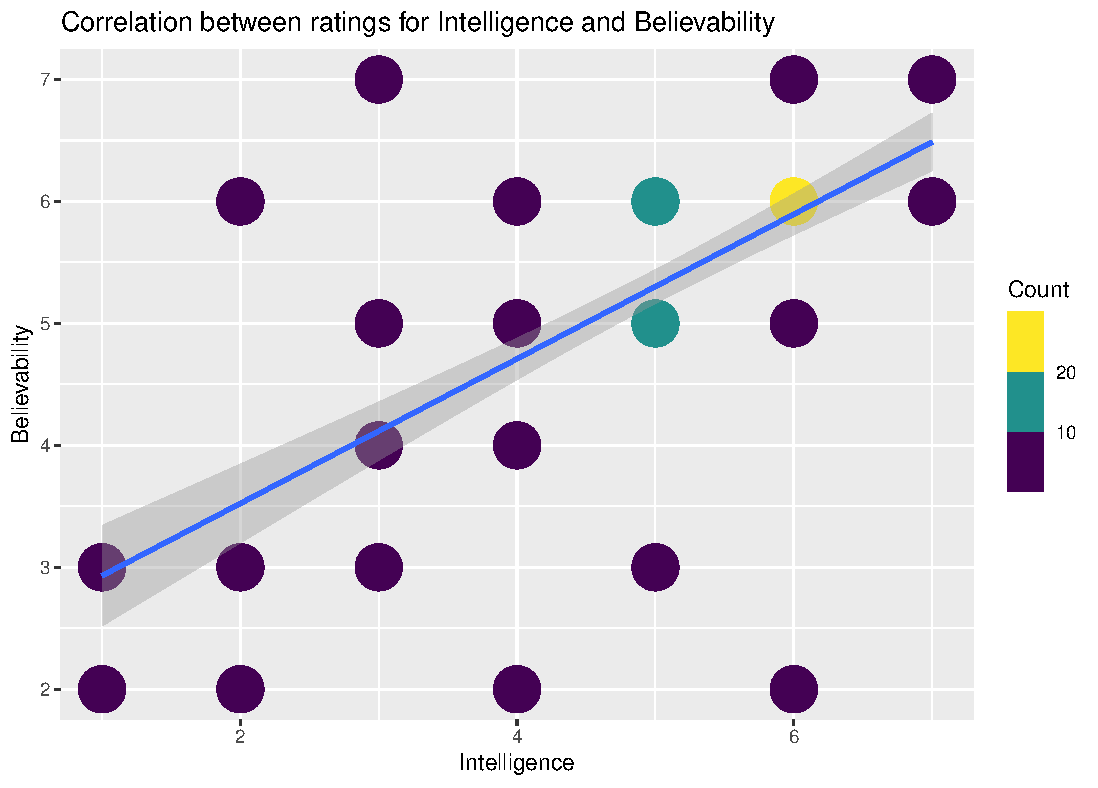
\includegraphics[width=\linewidth]{Images/Graphs/PH2IntelBelieveScatter.pdf}
  
\caption{Scatter plot displaying the correlation between intelligence and believabilty}
\label{fig:PH2IntelBelieveScatter}
\end{figure}

\section{Discussion}
\label{Discussion}

Does the use of adaptive AI help to build player-companion collaboration?

The results show very little difference perceived between both companion agents. Many of the box plots and bar charts show near identical perceptions between agent types. Pairwise comparisons were used to further examine any differences, and many responses indicate that there was no difference perceived between each agent type for all of the metrics the agents were measured on.

This would suggest that implementing adaptive behaviours via agent modelling may not be suitable for a real time action game. Many of the players perceived little difference and this could be that they were focusing on their own enemies too much to notice the companions’ actions.

The players could have also perceived the random behaviour changes in the IT agent as adaptive behaviour, even if the agent was not actually adapting to player actions. When playing in a high tense action setting, the player may not be able to notice what behaviours the AI adapts to. However, the regular behaviour changes could have been perceived as adaptive behaviour because it appears as though they are changing their behaviour. This corroborates with Brown’s views on good AI, where the AI needs to make the reasons for its behaviour obvious because the player does not know what’s going on behind the scenes \cite{GMTGoodAI}.

The last issue could have been the lack of time spent with each companion type. In such a short amount of time, the player may not be given the chance to learn how the AI adapts to their own behaviour. This could be better in a full game setting, where the player might be able to learn how the AI adapts and use it better as an advanced game mechanic, as opposed to a short combat demo.

%TODO High: Looking at the correlations between Collaboration/ UX and Adaptivity/ Collaboration
%Moderate correlation between collaboration and user experience
%Moderate correlation between adaptivity and collaboration

There was also some qualitative feedback from the surveys, and there were a lot of contrasting opinions on the behaviours like drawing enemies away or moving in between enemies and the player when they are struggling. Some players liked this kind of behaviour, remarking that “it felt like it had my back” for the AM companion and it “felt like it took more of the enemies away from me”. However this was also intrusive for some players. One player stated that the IT companion “Kept swooping in to help me when I didn’t want it to”. 

A lot of players had a greater mix of criticisms about the IT companion. Some stated that it was “Frustrating how quickly it changed enemies so often” or that it was “quite bad at properly focusing its attention on the right enemies”. However others thought it was “more intelligent… as it was able to split the group of enemies up evenly” or it “adapted to my playstyle”. This mix of opinions could have been caused by the random behaviour changes, as it may have randomly chosen behaviours the players found helpful, or chosen behaviours at the wrong time and so felt intrusive. On the other hand, the feedback for the AM companion seems more consistent. Despite this qualitative feedback, the test results show no perceivable difference between the AI companions.

%TODO Mid (Perform qualitative analysis)
%https://www.youtube.com/watch?v=wGQOvXF0Qr8
%https://www.youtube.com/watch?v=Zyu9cm4ui2c

The changes between the companions’ behaviour are also very subtle. Since one of the design goals was to make an AI agent that was generic enough to be used in various action games, all of the behaviours they perform are based on positioning (flanking, interposing or drawing enemies away). These provide only a slight differences between the different AI states, which are barely noticeable by the player. One player also suggested “(It) would be helpful if its actions were telegraphed somewhat, like through bark lines or colour indicators”, which is also mentioned by Brown and Naughty Dog developers \cite{GMTGoodAI, GAIP2EllieAI}. Using vocal barks would help distinguish similar behaviours as the AI could explain their actions or reasoning. Colour indicators or UI elements may not be as obvious in fast paced action games, but may be better suited for lower budget games, which was one of the other design goals in this research.

Future proofing is another consideration. Even though the IT agent was easier to implement, it would also be impossible to polish for a commercial product since the AI designer cannot make changes to the agent’s considerations, only the behaviours it can make. If the AI has access to special abilities, such as healing the player, it would not be possible for the IT companion to determine when to use them, since its actions are random. Alternatively, the AM agent can use the player state to determine when it would be the best time to use these abilities. In games with these types of actions, the AM companion may be preferred.

Some players felt overshadowed by their companions. Section (Ref) describes techniques Naughty Dog used to address these issues while still making the AI seem active in the fight. Alternatively, maybe an idle state could be added to the player model, where the AI will try to move closer to the player to keep them more engaged in the fight.

\subsection{Limitations}
\label{Limitations}

One of the key limitations was the choice to keep the AI agents generic by omitting having special abilities or vocal barks for the companions. This choice was made to focus the research on the player modelling technique, and to focus on providing an generic agent that can be scaled up to include these elements, but does not rely on them.

However, these limitations made it difficult to design unique behaviours for various states that were noticeable since the only way to distinguish them was through positioning. In this research, the differences in the behaviours were too subtle for the players to notice and it was not clear why they were making specific choices.

The play time for the experiment should have been slightly longer. A small combat scenario may not have been enough for the players to notice any differences. However, in a longer session, the player may have the chance to discover the companions’ behaviour and learn how the agents respond to their strategies.

The experiment should have also been structured more intuitively. Instead of asking the participants to fill out the questions for both companions after playing with both of them, the questions should have been filled out for each companion one at a time. This would reduce the number of incorrectly filled questionnaires and remove any ambiguity that the participant filled in the questions for the wrong agent type. Additionally, the agents would be more fresh in their mind when they fill out the questionnaire.

The reference code should have been saved or copied to the clipboard. Some respondents had to play through the demo again to get a new reference code, which may have influenced their opinion on the AI.

There were also a concerning number of participants who put agree (6) down for most of the questions. This could have been the result of a slight bias where the participants put down answers that they thought the researcher wanted them to.

%TODO Mid: look further into this ^

Including more negative questions like “I thought this companion was boring” could help filter such responses and make the participants think more about each individual question. Additionally, the questions could have been rated on a slider, which would also increase the range. The 7-point likert scale was used because it allows the user multiple stages of agreeableness or disagreeableness, but participants tend to avoid extreme answers like strongly agree since it makes them appear zealous or they want to reserve extreme answers for future questions (cite). Using a slider scale may reduce this as there is much more variety in how much the participant can agree or disagree with the statement.

Another limitation would be the number of responses. The target number of 59 participants was met, however 4 responses had to be removed due to incorrectly filled surveys, so the number of valid responses is slightly below the target.

\subsection{Recommendations}
\label{Recommendations}

The agent modelling companion may perform better with behaviours that have a greater contrast between them. While some of the positioning behaviours implemented are useful for cooperating with the player, this can be extended with special abilities that allow the companion to heal the player, or perhaps restore resources for them if they fit for the game. Many games, such as God of War or Bioshock, allow companions to use supportive abilities to cooperate better with the player, and this agent modelling approach could be used to determine when these actions would have the most effect on the player \cite{AIGamesBioshockAI, GDCAtreus}

Alternatively, there could be some feedback to let the player know what the companion’s actions are and why they are making them. An effective way to implement this would be with voice lines since the companion could explain why they are taking their actions, but some players suggested visual feedback like changing colours. This may not be as obvious for the player though as they would need to be able to see the companion, and having to look away from the action to find out what their companion is doing may be too distracting in a real time action game. However, this may be preferable for silent games or those with smaller budgets.

More time could also be spent on refining the player model and behaviour trees. The feeling of being overshadowed by the companion could be reduced by tracking damage dealt or number of kills by the player and companion and using those stats in the player model to determine whether the agent is being too active. If it is, then they could use more supportive behaviours.

Additionally, there could be more behaviours in each state to increase variety if the player’s playstyle isn’t changing much. There was a feature that allowed the agent to switch to the next highest states if they stayed in the same state for too long, however having greater variety within each state would be easier to polish.

The environment and gameplay design may also have an effect on the AI. More complicated combat environment with obstacles and cover could have provided more considerations for the AI. In addition, including a variety of enemy types would encourage the player to change their strategies, allowing the player modelling companion to change their own playstyle to better reflect the new situation. The testing environment could have included a variety of combat scenarios with different enemy types and compositions, thus requiring the player to change their strategy. A similar method was used by Guckelsberger et al when testing their CEM AI \cite{CoupledEmpowermentMaximisation}. Though this would be able to evaluate the agents more accurately, this would have been a little out of scope for this experiment to implement.

Difficulty is another consideration for how useful players found the AI. In the initial prototype, the game was designed to be difficult to require the player to use strategy and see value in their companion. However, verbal feedback from the quality assurance testing, see section \ref{Validation}, showed that it was too frustrating and players were too busy to notice the companion, so the difficulty was reduced.

These changes may have made the game too easy, as the players did not have to think about strategy and button mashing became a viable strategy, which reduces how well the companion can adapt to the player. The easier difficulty also means that the players had more breathing room to notice and let the companion fight on its own, which is where some of them may have thought that it was overshadowing them.

A better balance in difficulty may have given the player the chance to notice the companion and not get frustrated, while also requiring the need for strategy. Additionally, a game with slower pacing would also make for a better environment for the AM companion since thee player gets more of a chance to notice their companion’s actions. Further research could be conducted to determine the effects of difficulty on the player’s perception of their companions.

\section{Further Work}
\label{Further Work}

Further work needed, one more iteration to improve the adaptive agent

As outlined in the previous section, the AM companion may have performed better if it had access to more complex behaviours and vocal barks to make its behaviours more obvious. Iterating on this companion by adding these elements would be an avenue for further research as it would show how the AM companion can be scaled up to include more complex features.

\section{Conclusions}
\label{Conclusions}

The results of the experiment show that the player modelling approach used has no perceivable impact on how collaborative players felt their companion was in a real time action game. Despite this, this research evaluates a technique that is usually used for strategy games in a real time action game, and presents an AI companion that can respond to player actions.

Even though players found no perceivable difference between the 2 agents tested in this research, the player modelling agent can be scaled up and polished for games, unlike the IT agent because it is impossible to fine tune random actions. The next section offers advice and further work that can be taken to fine tune and polish the player modelling companion to make it collaborate better with players.

\section*{Acknowledgments}

I would like to thank the staff at Falmouth University for their support. In particular, I'd like to thank my project supervisor, Joseph Walton-Rivers, for his guidance on the project, as well as Michael Scott, the module leader for the dissertation modules. I would also like to thank everyone that participated in the playtesting.

%I would also like to thank everyone that participated in the playtesting.

\bibliographystyle{IEEEtran}
\bibliography{bibliography} 

 \newpage

\onecolumn
\section{Appendices}
\label{Appendices}

\subsection{Appendix - Links}
\label{AppendixLinks}

This is the link to the Github Repository: \url{https://github.falmouth.ac.uk/Games-Academy-Student-Work-22-23/Buddy-NPC-Dissertation}

This is the link to the Microsoft Forms questionnaire \url{https://forms.office.com/Pages/ShareFormPage.aspx?id=s-4LVT1qRkahEfidAXd5LhYJGdgYND9Nn38bE3C1BhpUQVNUUkdQREdNWjQzV1BCRjE5MUUyOEZCTy4u&sharetoken=TNyfcCNSzhBCKWwSOgEt}

\subsection{Appendix - Quality Assurance Plan}
\label{AppendixQAPlan}
%(Perry 1987)
%Correctness, Reliability, Efficiency, Integrity, Usability, Maintainability, Testability, Flexibility, Portability, Interoperability

%Types of Testing: Unit Testing, Automation and Continuous Integration, Run-Time Analyses, End-User Testing

The artefact will be tested in multiple stages. First, the basic combat mechanics and enemy AI will be playtested with end-users, which would most likely be friends and family, to ensure that there are no bugs that could interfere with the results of the experiment. I will gather vocal feedback and track any issues on a Trello board, which will be used to mark progress.

This is an important aspect as the basic mechanics will determine how the player interacts with the game and the decision making for the companion agent relies on this.

When the basic combat mechanics and enemy AI are tested, the adaptive AI will go into testing. Unit tests will be used to confirm the calculations for generating the player model are correct and that the correct behaviours are chosen for the adaptive AI.

Once the adaptive agent has passed the unit testing, run-time testing will be used for optimisation. The aim is for the game to run at a minimum of 30 fps on the machines in the Games Academy. If the game isn't performant enough, the profiler in Unity will be used to find bottlenecks and fix them.

Before conducting the experiment, the game will be tested again with friends and family to ensure that the adaptive AI is behaving properly and to regulate difficulty. While game balance is not a primary concern here, the game should be challenging enough so that the companion provides clear use for the player, but not overwhelming to distract the player from noticing them.

Throughout this process, regular builds will be made and tested to ensure that it works. Automated build generation may be used to make this process quicker.

Additionally, generating reference codes will need to be tested to ensure that multiple participants will not be given the same code. The initial plan for constructing the reference code is to construct multiple sets of digits. The first set of digits could be the current time, then next set could be randomly generated and the final digits could be determined by which AI the participant was given first. This system will need to be tested properly when it is developed.

\newpage

\subsection{Appendix - R-Code}
\label{AppendixRCode}

%TODO High - Format R code properly

\begin{verbatim}

# Links for useful info ####

# LINK Essentials Course: https://www.linkedin.com/learning/r-essential-training-wrangling-and-visualizing-data/creating-tidy-data?autoplay=true&resume=false&u=56738929
# LINK GDC 3 Tests: https://www.youtube.com/watch?v=fl9V0U2SGeI&list=PLVmb_qp6XRcwzN9l5mcia6Gh3HOgut3bH&index=9
# LINK Correlation Tests Docs: https://www.rdocumentation.org/packages/stats/versions/3.6.2/topics/cor.test
# LINK Correlation Test Docs: https://bookdown.org/ndphillips/YaRrr/correlation-cor-test.html
# LINK Pearson Correlation Coefficient: https://en.wikipedia.org/wiki/Pearson_correlation_coefficient

# End Links ####

# Setup ####

## Setting up the libraries ====
library(tidyverse)
library(psych)
library(readr)
library(ggplot2)
library(MASS)
library(broom)
library(hexbin)
library(dplyr)
library(ggpointdensity)

## Setting up data ====

### Getting the data, view gets data file but cannot be compiled ----
rawData <- read_csv("DataResults.csv")
glimpse(rawData)

### Replace the labels ----
factorData <- rawData %>%
  mutate(AgentType = factor(AgentType, levels = c("AM", "IT"),
                            labels = c("Agent Modelling", "Interval Timing"))) %>%
  mutate(Success = factor(Success, levels = c("Agree", "Disagree"),
                            labels = c("Success", "Fail"))) %>%
  mutate(Believable = factor(Believable, levels = c("Strongly agree", "Agree", "Slightly agree", "Neither agree nor disagree", "Slightly disagree", "Disagree", "Strongly disagree"),
                            labels = c("7", "6", "5", "4", "3", "2", "1"))) %>%
  mutate(Intelligent = factor(Intelligent, levels = c("Strongly agree", "Agree", "Slightly agree", "Neither agree nor disagree", "Slightly disagree", "Disagree", "Strongly disagree"),
                               labels = c("7", "6", "5", "4", "3", "2", "1"))) %>%
  mutate(ChangePlay = factor(ChangePlay, levels = c("Strongly agree", "Agree", "Slightly agree", "Neither agree nor disagree", "Slightly disagree", "Disagree", "Strongly disagree"),
                                labels = c("7", "6", "5", "4", "3", "2", "1"))) %>%
  mutate(LikeChange = factor(LikeChange, levels = c("Strongly agree", "Agree", "Slightly agree", "Neither agree nor disagree", "Slightly disagree", "Disagree", "Strongly disagree"),
                               labels = c("7", "6", "5", "4", "3", "2", "1"))) %>%
  mutate(Effective = factor(Effective, levels = c("Strongly agree", "Agree", "Slightly agree", "Neither agree nor disagree", "Slightly disagree", "Disagree", "Strongly disagree"),
                               labels = c("7", "6", "5", "4", "3", "2", "1"))) %>%
  mutate(Overshadowed = factor(Overshadowed, levels = c("Strongly agree", "Agree", "Slightly agree", "Neither agree nor disagree", "Slightly disagree", "Disagree", "Strongly disagree"),
                              labels = c("7", "6", "5", "4", "3", "2", "1"))) %>%
  mutate(Collaboration = factor(Collaboration, levels = c("Strongly agree", "Agree", "Slightly agree", "Neither agree nor disagree", "Slightly disagree", "Disagree", "Strongly disagree"),
                            labels = c("7", "6", "5", "4", "3", "2", "1"))) %>%
  mutate(Adapted = factor(Adapted, levels = c("Strongly agree", "Agree", "Slightly agree", "Neither agree nor disagree", "Slightly disagree", "Disagree", "Strongly disagree"),
                                 labels = c("7", "6", "5", "4", "3", "2", "1"))) %>%
  mutate(Enjoyed = factor(Enjoyed, levels = c("Strongly agree", "Agree", "Slightly agree", "Neither agree nor disagree", "Slightly disagree", "Disagree", "Strongly disagree"),
                            labels = c("7", "6", "5", "4", "3", "2")))

### Convert factors to numeric values ----

dblData <- factorData %>%
  mutate(Believable = 8 - as.integer(Believable)) %>%
  mutate(Intelligent = 8 - as.integer(Intelligent)) %>%
  mutate(ChangePlay = 8 - as.integer(ChangePlay)) %>%
  mutate(LikeChange = 8 - as.integer(LikeChange)) %>%
  mutate(Effective = 8 - as.integer(Effective)) %>%
  mutate(Overshadowed = 8 - as.integer(Overshadowed)) %>%
  mutate(Collaboration = 8 - as.integer(Collaboration)) %>%
  mutate(Adapted = 8 - as.integer(Adapted)) %>%
  mutate(Enjoyed = 8 - as.integer(Enjoyed))
    # The ratings get reversed when converted to a numeric value
    # So subtracting them away from 8 reverts them to their normal value

glimpse(dblData)

### Replace null values with 4 (midpoint) ----

data <- dblData

  data$Believable[is.na(data$Believable)] <- 4
  data$Intelligent[is.na(data$Intelligent)] <- 4
  data$ChangePlay[is.na(data$ChangePlay)] <- 4
  data$LikeChange[is.na(data$LikeChange)] <- 4
  data$Effective[is.na(data$Effective)] <- 4
  data$Overshadowed[is.na(data$Overshadowed)] <- 4
  data$Collaboration[is.na(data$Collaboration)] <- 4
  data$Adapted[is.na(data$Adapted)] <- 4
  data$Enjoyed[is.na(data$Enjoyed)] <- 4

glimpse(data)

### Creates a data frame for mean values and standard deviation ----
sumData <- data %>%
  group_by(AgentType) %>%
  summarize(enjoyMean = mean(Enjoyed),
            enjoyError = sd(Enjoyed)/sqrt(n()),
            
            intelligenceMean = mean(Intelligent),
            intelligenceError = sd(Intelligent)/sqrt(n()),
            
            adaptabiltyMean = mean(Adapted),
            adaptabiltyError = sd(Adapted)/sqrt(n()),
            
            sampleCount = n())%>%
  ungroup()

sumData

### Group Data by Agent Type ----
AMData <- subset(data, AgentType == "Agent Modelling")

AMData

ITData <- subset(data, AgentType == "Interval Timing")

ITData


## Qualitative data ====

qualitativeData <- read_csv("QualitativeDataResults.csv")
glimpse(qualitativeData)

# End Setup ####


# Statistical Tests ####

## T Test for Hypothesis 1 - Adaptive companion will seen as more collaborative compared to the non adaptive companion ====

collabTest <- t.test(AMData$Collaboration, ITData$Collaboration, 
                     alternative="greater")
collabTest

## Correlation Test for Hypothesis 2 - Players' user experience will be improved if they felt a greater sense of collaboration ====

uxTest <- cor.test(data$Enjoyed, data$Collaboration,
                   method = c("pearson"))
uxTest

## Correlation Test for Posthoc Hypothesis 1 - Players will rate their agent as more collaborative if they thought they were more adaptive ====

adaptiveTest <- cor.test(data$Adapted, data$Collaboration,
                       method = c("pearson"))
adaptiveTest

## Correlation Test for Posthoc Hypothesis 2 - Players will rate their agent as more believable if they thought they were more intelligent ====

believableTest <- cor.test(data$Intelligent, data$Believable, method = c("pearson"))

believableTest

# End Statistical Tests ####

# Visualising Basic Data ####


data %>%
  group_by(AgentType) %>%
  summarise(min = min(LikeChange), median = median(LikeChange), max = max(LikeChange))

data %>%
  group_by(AgentType) %>%
  summarise(min = min(Intelligent), median = median(Intelligent), max = max(Intelligent))
## Box Plots ====

qplot(factor(data$AgentType), data$Effective, geom = "boxplot", 
      main="Comparing the combat effectiveness rating of the companions", 
      xlab="AI Type", ylab="Combat Effectiveness")

qplot(factor(data$AgentType), data$Intelligent, geom = "boxplot", 
      main="Comparing the intelligence rating of the companions", 
      xlab="AI Type", ylab="Intelligence")

qplot(factor(data$AgentType), data$Collaboration, geom = "boxplot", 
      main="Comparing the collaboration rating of the companions", 
      xlab="AI Type", ylab="Collaboration")

qplot(factor(data$AgentType), data$Adapted, geom = "boxplot", 
      main="Comparing the adaptivity rating of the companions", 
      xlab="AI Type", ylab="Adaptivity")

qplot(factor(data$AgentType), data$Enjoyed, geom = "boxplot", 
      main="Comparing how much players enjoyed playing with each companions", 
      xlab="AI Type", ylab="Enjoyed Playing")


## Bar Charts to show distribution ====

ggplot(data=data, aes(Effective, fill=AgentType)) +
  geom_bar(position = position_dodge(), colour = "black") +
  labs(title = "Distribution of user ratings for combat effectiveness",
       x = "Combat Effectiveness", y = "Count")

ggplot(data=data, aes(Intelligent, fill=AgentType)) +
  geom_bar(position = position_dodge(), colour = "black") +
  labs(title = "Distribution of user ratings for intelligence",
       x = "Intelligence", y = "Count")

ggplot(data=data, aes(Collaboration, fill=AgentType)) +
  geom_bar(position = position_dodge(), colour = "black") +
  labs(title = "Distribution of user ratings for collaboration",
       x = "Collaboration", y = "Count")

ggplot(data=data, aes(Adapted, fill=AgentType)) +
  geom_bar(position = position_dodge(), colour = "black") +
  labs(title = "Distribution of user ratings for adaptivity",
       x = "Adaptivity", y = "Count")

ggplot(data=data, aes(Enjoyed, fill=AgentType)) +
  geom_bar(position = position_dodge(), colour = "black") +
  labs(title = "Distribution of user ratings for how much they enjoyed playing with this companion",
       x = "Enjoyed Playing", y = "Count")

## Bar Charts to compare ratings ====

ggplot(data=data, aes(Collaboration)) +
  geom_bar(position = position_dodge(), colour = "black") +
  labs(title = "Normal distribution of user ratings for collaboratoin",
       x = "Collaboration", y = "Count")

ggplot(data=data, aes(Effective)) +
  geom_bar(position = position_dodge(), colour = "black") +
  labs(title = "Normal distribution of user ratings for combat effectiveness",
       x = "Combat Effectiveness", y = "Count")

# End Visualising Basic Data ####

# Mapping Data ####
## Adaptivity, Intelligence and Believability ----

qplot(data$Adapted, data$Intelligent, geom = c("point", "smooth"), method = "rlm",
      main = "Correlation between ratings for Adaptivity and Intelligence", 
      xlab = "Adaptivity", ylab = "Intelligence")

ggplot(data, aes(x = Adapted, y = Intelligent)) +
  geom_pointdensity(size = 10) +
  scale_color_viridis_b() + 
  geom_smooth(method = 'rlm', se = TRUE) +
  labs(title = "Correlation between ratings for Adaptivity and Intelligence",
       x = "Adaptivity", y = "Intelligence", colour = "Count")

cor(data$Adapted, data$Intelligent, method = c("pearson"))

qplot(data$Intelligent, data$Believable, geom = c("point", "smooth"), method = "rlm",
      main = "Correlation between ratings for Intelligence and Believability", 
      xlab = "Intelligence", ylab = "Believability")

ggplot(data, aes(x = Intelligent, y = Believable)) +
  geom_pointdensity(size = 10) +
  scale_color_viridis_b() + 
  geom_smooth(method = 'rlm', se = TRUE) +
  labs(title = "Correlation between ratings for Intelligence and Believability",
       x = "Intelligence", y = "Believability", colour = "Count")

cor.test(data$Intelligent, data$Believable, method = c("pearson"))

qplot(data$Adapted, data$Believable, geom = c("point", "smooth"), method = "rlm",
      main = "Correlation between ratings for Adaptivity and Believability", 
      xlab = "Adaptivity", ylab = "Believability")

ggplot(data, aes(x = Adapted, y = Believable)) +
  geom_pointdensity(size = 10) +
  scale_color_viridis_b() + 
  geom_smooth(method = 'rlm', se = TRUE) +
  labs(title = "Correlation between ratings for Adaptivity and Believability",
       x = "Adaptivity", y = "Believability", colour = "Count")

cor(data$Adapted, data$Believable, method = c("pearson"))

## Adaptivity, Collaboration and Combat Effectiveness ----

ggplot(data, aes(x = Adapted, y = Collaboration)) +
  geom_pointdensity(size = 10) +
  scale_color_viridis_b() + 
  geom_smooth(method = 'rlm', se = TRUE) +
  labs(title = "Correlation between ratings for Adaptivity and Collaboration",
       x = "Adaptivity", y = "Collaboration", colour = "Count")

cor(data$Adapted, data$Collaboration, method = c("pearson"))

ggplot(data, aes(x = Collaboration, y = Effective)) +
  geom_pointdensity(size = 10) +
  scale_color_viridis_b() + 
  geom_smooth(method = 'rlm', se = TRUE) +
  labs(title = "Correlation between ratings for Collaboration and Combat Effectiveness",
       x = "Collaboration", y = "Combat Effectiveness", colour = "Count")

cor(data$Collaboration, data$Effective, method = c("pearson"))

ggplot(data, aes(x = Adapted, y = Effective)) +
  geom_pointdensity(size = 10) +
  scale_color_viridis_b() + 
  geom_smooth(method = 'rlm', se = TRUE) +
  labs(title = "Correlation between ratings for Adaptivity and Combat Effectiveness",
       x = "Adaptivity", y = "Combat Effectiveness", colour = "Count")

cor(data$Adapted, data$Effective, method = c("pearson"))

## Overshadowing, Combat Effectiveness and Enjoyed Playing ----

qplot(data$Overshadowed, data$Enjoyed, geom = c("point", "smooth"), method = "rlm",
      main = "Correlation between ratings for Overshadowing and how much they enjoyed playing", 
      xlab = "Overshadowing", ylab = "Enjoyed Playing")

ggplot(data, aes(x = Overshadowed, y = Enjoyed)) +
  geom_pointdensity(size = 10) +
  scale_color_viridis_b() + 
  geom_smooth(method = 'rlm', se = TRUE) +
  labs(title = "Correlation between ratings for Overshadowing and how much they enjoyed playing",
       x = "Overshadowing", y = "Enjoyed Playing", colour = "Count")

cor(data$Overshadowed, data$Enjoyed, method = c("pearson"))

qplot(data$Overshadowed, data$Effective, geom = c("point", "smooth"), method = "rlm",
      main = "Correlation between ratings for Overshadowing and Combat Effectiveness", 
      xlab = "Overshadowing", ylab = "Combat Effectiveness")

ggplot(data, aes(x = Overshadowed, y = Effective)) +
  geom_pointdensity(size = 10) +
  scale_color_viridis_b() + 
  geom_smooth(method = 'rlm', se = TRUE) +
  labs(title = "Correlation between ratings for Overshadowing and Combat Effectiveness",
       x = "Overshadowing", y = "Combat Effectiveness", colour = "Count")

cor(data$Overshadowed, data$Effective, method = c("pearson"))

qplot(data$Effective, data$Enjoyed, geom = c("point", "smooth"), method = "rlm",
      main = "Correlation between ratings for Combat Effectiveness and how much they enjoyed playing", 
      xlab = "Combat Effectiveness", ylab = "Enjoyed Playing")

ggplot(data, aes(x = Effective, y = Enjoyed)) +
  geom_pointdensity(size = 10) +
  scale_color_viridis_b() + 
  geom_smooth(method = 'rlm', se = TRUE) +
  labs(title = "Correlation between ratings for Combat Effectiveness and how much they enjoyed playing",
       x = "Combat Effectiveness", y = "Enjoyed Playing", colour = "Count")

cor(data$Effective, data$Enjoyed, method = c("pearson"))

## Collaboration and User Experience ====

ggplot(data, aes(x = Collaboration, y = Enjoyed)) +
  geom_pointdensity(size = 10) +
  scale_color_viridis_b() + 
  geom_smooth(method = 'rlm', se = TRUE) +
  labs(title = "Correlation between ratings for Collaboration and how much they enjoyed playing",
       x = "Collaboration", y = "Enjoyed Playing", colour = "Count")

# End Mapping Data ####

# Pairwise Comparisons ####

## Setting Up Data ====

pairData <- subset(data, AgentType == "Interval Timing")

pairData$AgentType = "Comparison"
pairData$Believable = pairData$Believable - AMData$Believable
pairData$Intelligent = pairData$Intelligent - AMData$Intelligent
pairData$ChangePlay = pairData$ChangePlay - AMData$ChangePlay
pairData$LikeChange = pairData$LikeChange - AMData$LikeChange
pairData$Effective = pairData$Effective - AMData$Effective
pairData$Overshadowed = pairData$Overshadowed - AMData$Overshadowed
pairData$Collaboration = pairData$Collaboration - AMData$Collaboration
pairData$Adapted = pairData$Adapted - AMData$Adapted
pairData$Enjoyed = pairData$Enjoyed - AMData$Enjoyed

pairData

## Graphs ====

ggplot(data=pairData, aes(Believable)) +
  geom_bar(position = position_dodge(), colour = "black") +
  labs(title = "Difference between believability ratings for each agent",
       x = "Believability", y = "Count")

ggplot(data=pairData, aes(Intelligent)) +
  geom_bar(position = position_dodge(), colour = "black") +
  labs(title = "Difference between intelligence ratings for each agent",
       x = "Intelligence", y = "Count")

ggplot(data=pairData, aes(ChangePlay)) +
  geom_bar(position = position_dodge(), colour = "black") +
  labs(title = "Difference between ratings for how each agent caused the player to change their playstyle",
       x = "Combat Effectiveness", y = "Count")

ggplot(data=pairData, aes(LikeChange)) +
  geom_bar(position = position_dodge(), colour = "black") +
  labs(title = "Difference between ratings for how much the player liked that their own playstyle changed for each agent",
       x = "Combat Effectiveness", y = "Count")

ggplot(data=pairData, aes(Effective)) +
  geom_bar(position = position_dodge(), colour = "black") +
  labs(title = "Difference between combat effectiveness ratings for each agent",
       x = "Combat Effectiveness", y = "Count")

ggplot(data=pairData, aes(Overshadowed)) +
  geom_bar(position = position_dodge(), colour = "black") +
  labs(title = "Difference between ratings for how overshadowing each agent was",
       x = "Overshadowing", y = "Count")

ggplot(data=pairData, aes(Collaboration)) +
  geom_bar(position = position_dodge(), colour = "black") +
  labs(title = "Difference between collaboration ratings for each agent",
       x = "Collaboration", y = "Count")

ggplot(data=pairData, aes(Adapted)) +
  geom_bar(position = position_dodge(), colour = "black") +
  labs(title = "Difference between adaptivity ratings for each agent",
       x = "Adaptivity", y = "Count")

ggplot(data=pairData, aes(Enjoyed)) +
  geom_bar(position = position_dodge(), colour = "black") +
  labs(title = "Difference between ratings for how much players enjoyed playing with each agent",
       x = "Enjoyed Playing", y = "Count")

# End Pairwise Comparisons ####

# Qualitative Data ####
## Graphs ====


ggplot(data=qualitativeData, aes(Opinion, fill=AgentType)) +
  geom_bar(position = position_dodge(), colour = "black") +
  labs(title = "Distribution of user ratings for combat effectiveness",
       x = "Combat Effectiveness", y = "Count")



\end{verbatim}

\newpage

\subsection{Appendix - Graphs with Random Data}

%TODO mid - ask michael if these can be removed

Figures \ref{fig:LikabilityRplot} and \ref{fig:IntelligenceLikabilityRplot} have been created using the R-Code in appendix \ref{AppendixRCode}. Random data has been put into these graphs to show a sample of what the graphs would look like.

Figure \ref{fig:LikabilityRplot} displays a box plot that compares the likability between the 2 agent types while figure \ref{fig:IntelligenceLikabilityRplot} shows a q plot that displays how the perceived intelligence of the AI relates to the ranking for likability.

\label{AppendixGraphs}
\begin{figure}[h!]
  \centering
  \includegraphics[width=0.9\linewidth]{Images/Sample Graphs/LikabilityRplot.png}
  
\caption{Comparing the likability between companion types (sample data)}
\label{fig:LikabilityRplot}
\end{figure}

\begin{figure}[h!]
  \centering
  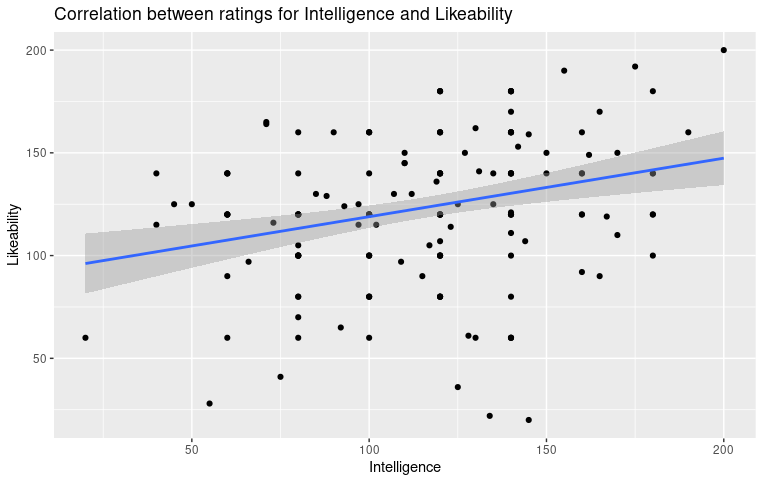
\includegraphics[width=0.9\linewidth]{Images/Sample Graphs/IntelligenceLikabilityRplot.png}
  
\caption{Comparing the effect perceived intelligence has on likability (sample data)}
\label{fig:IntelligenceLikabilityRplot}
\end{figure}

\end{document}